% siminos/blog/2modesBB.tex
% $Author$ $Date$

% Predrag 2013-08-10 Burak, git version only

\noindent
{\color{red} Do edit this git file (created 2013-08-10),
it is a new addition to the original svn version (which for now
stays untouched, the mother version is still the svn one).
}
\bigskip\bigskip

\subsection{{\twoMode} writeup}
\label{chap:2modesBBproj}

\begin{description}

\item[2013-07-25  Predrag] This is \BBedit{an example of Burak's edit},
and here is an internal footnote\BB{An internal footnote by Burak.}. They
are useful when you change something n the middle of a text, rather then
just append the newest blog post. Please remove the color from my
\PCedit{edits} as you read them and approve them, and I'll do the same
for yours.

% \item[2013-08-13  Predrag to Burak] Please define \eqv, \reqv, \po,
% and \rpo\ here, in form suitable for pasting into the putative
% \twoMode\ slicing paper.

    \PCedit{
\item[2013-08-14  Predrag]
Your definition of a \reqv\ is correct for one-parameter $\Group$, but we
will have to rethink it for $N$\dmn\ Lie group $\Group$. In that case the
time trajectory is a 1\dmn\ curve, generically tracing out the $N$\dmn\
group orbit quasiperiodically. Probably a
\HREF{http://www.streamsound.dk/book1/chaos/chaos.html\#205/z} {better
definition} (click on magenta hyperlinks!) would be that
$\vel({\ssp_{\ssp}}) \in \pS_{EQ}$, and than show that this is then true
true anywhere on the group orbit. Perhaps using
\HREF{http://www.streamsound.dk/book1/chaos/chaos.html\#204/z} {Lie
derivatives}...
    }

\end{description}

% [2013-08-13 Burak]
\noindent{\bf Invariant solutions:}                     \toCB
A point $\ssp_{EQ}$ is an \eqv\ if the velocity function evaluated at this
point is 0, namely, $\dot{\ssp}|_{\ssp=\ssp_{EQ}} = \vel({\ssp_{EQ}}) = 0$.
Orbit of
a point $\ssp$ of a $\Group$-equivariant flow is called a \reqv\ if for any
time evolved point on the orbit $\ssp(\tau) = f^{\tau}(\ssp_{REQ})$ there
exists a parameter $\phi$ such that $\ssp(\tau) = \Group(\phi) \ssp$, in other
words, a time orbit is a \reqv\ if it coincides with the group orbit.
 A
point $\ssp$ is on a \po\ if its trajectory passes through itself after some
certain time \period{}, namely $\ssp = f^{\period{}}(\ssp)$. Finally, a point $\ssp$ of a
$\Group$-equivariant flow is said to be on a \rpo\ if there exists a
point $\ssp(\period{}) = f^\period{}(\ssp)$ on the orbit of $\ssp$, such that it satisfies $\ssp(\period{}) =
\LieEl(\phi) \ssp$ for a certain $\phi$.

\noindent{\bf A truncation of PDE representations:}
The {\twoMode} system is the simplest, coarsest example of a truncation
of a Fourier representation of a PDEe. Consider, for example, the $1D$
\KSe.
%
\PC{2013-08-13 Predrag copied this from \refref{SCD07}, to set up
the conventions for the \KSe\ calculations.}
%
The time evolution of the `flame front velocity'
$u=u(x,t)$ on a periodic domain $u(x,t) = u(x+L,t)$ is given by
\beq
  u_t = F(u) = -{\textstyle\frac{1}{2}}(u^2)_x-u_{xx}-u_{xxxx}
    \,,\qquad   x \in [-L/2,L/2]
    \,.
\ee{BBks}
Here $t \geq 0$ is the time, and $x$ is the spatial coordinate.
The subscripts $x$ and $t$ denote partial derivatives with respect to
$x$ and $t$. In what follows
we shall state results of all calculations either in units of the
`dimensionless system size' $\tildeL$, or the system size $L = 2 \pi
\tildeL$. All numerical results presented in this report
are for $\tildeL=22/2\pi \simeq 3.5014$.
Spatial periodicity $u(x,t)=u(x+L,t)$
makes it convenient to work in the Fourier space,
\beq
  u(x,t)=\sum_{k=-\infty}^{+\infty} a_k (t) e^{ i k x /\tildeL }
\,,
\ee{BBeq:ksexp}
with the $1$-dimensional PDE \refeq{ks}
replaced by an infinite set of
ODEs for the complex Fourier coefficients $a_k(t)$:
\beq
\dot{a}_k= \pVeloc_k(a)
     = ( q_k^2 - q_k^4 )\, a_k
    - i \frac{q_k}{2} \sum_{m=-\infty}^{+\infty} a_m a_{k-m}
\,,
\ee{BBexpan}
where $q_k = k/\tildeL$.
Since $u(x,t)$ is real, $a_k=a_{-k}^\ast$, and we can replace the
sum by a $k > 0$ sum. In the {\twoMode} system we keep only the
$k \in \{\pm 1,pm 2\}$ terms. This is very wrong as an approximation to
the \KSe, but --in the spirit of the Lorentz equations-- OK for hoping
to learn something about the qualitative dynamics of this class of
PDEs.



\subsection{Burak's {\twoMode} blog}
\label{chap:2modesBBblog}

\begin{description}
\item[2012-05-07  Predrag to Chaos Gang] It's not over until it is over.

\item[2013-07-25  Predrag]
 - instead of computing \cLf\ one more
time, how about giving a try to \twoMode\ $\SOn{2}$-equivariant flow,
defined in
\\
\texttt{reducesymm/cgang/2modes.tex}
\\ (you can get it by a click
\HREF{../cgang/2modes.pdf}{here}, provided you had already pdflatex-ed
2modes.tex). Have a look at it, and then meet with Daniel Borrero, 3. floor
Schatz lab, who can walk you through what we had already done and learned
(all in the 2modes.pdf blog). You can play with it for -let's say- two
weeks, see whether you can find an interesting strange attractor worth
slicing. If that does not work out, we'll give up, and go to \KS\ instead,
which is much more important for our overall goals...

\item[2013-08-06 Predrag]
A more precise statement of what we are trying to achieve with this model is
in \emph{reducesymm/cgang/2modes.tex:}

``For the 4\dmn\ model at hand are using the invariant polynomials
$\{u,v,w,q\}$ dynamics only to develop intuition, but to illustrate the
general \mslices, everything has to do be done in $\pS =
\{x_1,x_2,y_1,y_2\}$ and \slice\ $\pSRed$ as well. You can see that even
for the simplest conceivable $\SOn{2}$ 4-dimensional flow one has to
think about how to construct the invariant polynomial basis, and it is
hard to imagine how anyone could do that for very high\dmn\ flows.''

If we can find a nice strange attractor with comparable amplitudes in the
two modes, and show how to slice it, that would be the simplest example of
power of slicing, as the symmetry-reduced dynamics is 3\dmn\ and something
a human can look at, turn around as 3\dmn\ Mathematica or Matlab figure.

If in addition it turns out that my favorite Sobolev norm (read
\texttt{reducesymm/blog/norms.tex}) reduces the number of local slice
hyperplanes needed to cover the attractor, I'll be doubly happy.

\begin{figure}[ht]
\begin{center}
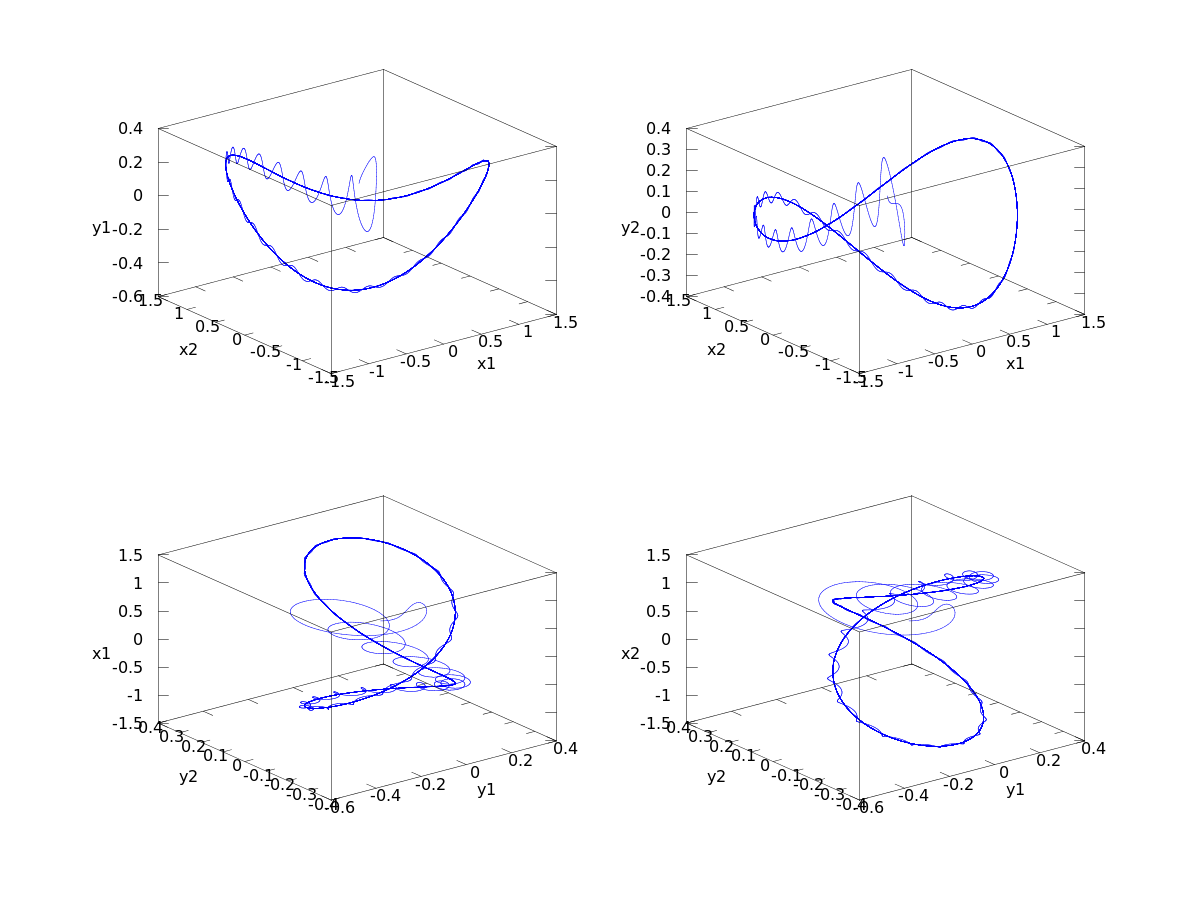
\includegraphics[width=0.9\textwidth]{PKperorb}
\end{center}
\caption{A typical
%Predrag 2013-08-05 removed ``periodic orbit''
attractive \reqv\  of \twoMode\ flow.}
\label{fig:PKperorb}
\end{figure}

\item[2013-08-05  Burak] I read the \twoMode\ blog and
    \HREF{http://chaosbook.org/paper.shtml\#stability} {Chapter 4} -
    {\em Local stability}, confirmed most of the findings in blog,
    naively experimented on the parameters of the system in $x_i, y_i$
    basis tried to find equilibria, got nothing, then talked to Daniel,
    and re-read the blog and come up with a Monte-Carlo (kind of)
    algorithm hoping that it could get me a strange attractor. So far,
    I only got periodic orbits. \refFig{fig:PKperorb} is a typical one.

\item[2013-08-06 Predrag]
Got worried that there were no updates for 11 days - how about if agree
on a schedule, let's say git pushes
\textcolor[rgb]{1.00,0.00,0.00}{every Monday and Friday}?

                                            \toCB
The \po s (actually, \reqva) that you find are presumably \emph{limit
cycles}. In ChaosBook I define `limit cycles' as \po s which are strictly
exponentially attracting forward in time. Parenthetically, in her thesis
De Witte\rf{DWRGK13,DeWitte13} defines a `limit cycle' as an ``isolated
periodic orbit'' thusly:

``A cycle of a continuous-time dynamical system, in a neighbourhood of
which there are no other cycles, is called a limit cycle.''

That presumably has advantage of being true for both directions of time,
but I do not think we need to get that finicky...


\item[2013-08-05  Burak]
    Here is what I did:
\begin{itemize}
\item
Generate pseudo-random set of parameters ensuring $\mu_1 > -\mu_2 > 0$, $c_1 = 1$ and $c_2 = -1$ as suggested in [2012-04-29 Predrag] and [2012-08-06 Edgar Knobloch]
\item
Numerically compute roots of \refeq{PKinvEqs5a} in $u>0, v>0$ region
starting from pseudo-random pair of points $(u,v)$, to find an
equilibrium in invariant polynomial basis.
\bea
\tilde{f}(\tilde{u},\tilde{v}) &=&
  \tilde{u}\,A_1 - \tilde{v}\,A_2 = 0 %Double checked DB 04-30-2012
\,,\qquad\qquad\qquad\qquad  deg(f) = 2
\continue
\tilde{g}(\tilde{u},\tilde{v}) &=&  %Double checked DB 04-30-2012
 \left(A_1^2
 - c_1\,\tilde{v}\right)
 \left(\tilde{u}+2\,\tilde{v}\right)^2
 +e_2^2\,\tilde{v}^2 = 0
\,,\qquad  deg(g) = 4
\continue
&& \mbox{where }
A_1 = \mu_1+\tilde{a_1}\,\tilde{u}+\tilde{b_1}\,\tilde{v},
\continue
&& \,\,\,\,\qquad A_2 = \mu_2+\tilde{a_2}\,\tilde{u}+\tilde{b_2}\,\tilde{v}
\,.
\label{PKinvEqs5a}
\eea
\item
Calculate corresponding w and q and check if the syzygy holds (it does).
\item
Calculate eigenvalues of the stability matrix at this point.
\item
If the stability matrix has at least one eigenvalue with positive real part (repulsive), at least one eigenvalue with negative real part (attractive) and a complex pair of eigenvalues with non-zero imaginary part (spiral); keep the parameters and the equilibrium point.
\item
Numerically calculate the points $x_i, y_i$ corresponding to the equilibrium in invariant polynomial basis, using following relations:
\bea
  u &=& x_1^2 + x_2^2\,,
\continue
  v &=& y_1^2 + y_2^2\,,
\continue
  w &=& 2x_1^2y_1+4x_1x_2y_2 - 2x_2^2y_1\,,
\continue
  q &=& 2x_1^2y_2+4x_1x_2y_1 + 2x_2^2y_2\,.
\label{eq:PKinvxirels}
\eea
\item
Integrate the Porter - Knobloch velocity function to see time evolution in real coordinates.
\end{itemize}
So far, I got divergent solutions and periodic orbits using parameters that I found this way. My questions:
\begin{itemize}
\item
If I check the eigenvalues of the stability matrix for real coordinates,
I get 3 of the eigenvalues almost same with the ones I get for the
invariant polynomial basis, and one eigenvalue 0 (usually something less
then $10^{-4}$). This gives me the feeling of I am doing things correct,
however, I want to make more sense out of this. Is there a clear
discussion about how these eigenvalues remain unchanged under coordinate
transformations (I saw the discussion about traces in the blog, I
confirmed the result that traces of stability matrices in $u,v,w,q$ basis
and $\pS = \{x_1,x_2,y_1,y_2\}$ basis are not the same at the origin.).
\item
Is what I did reasonable at all? Is there any obvious wrong logic?
\item
Would you suggest any other restrictive criteria to pick a ``good'' set of parameters, in addition to the ones I force on eigenvalues of the stability matrix? I thought, maybe I should take parameters for which the positive and negative real-part eigenvalues are of the same order.
\item
Is an equilibrium in invariant polynomial basis ($u,v,w,q$) a \reqv\ in
the full \statesp\ $\pS = \{x_1,x_2,y_1,y_2\}$ basis? ({\bf [2013-08-13 Predrag]} correct, it is.)
If not, what sense I should make out of the fact
that the relations \refeq{eq:PKinvxirels} do not provide a unique point
$\pS = \{x_1,x_2,y_1,y_2\}$ for given ($u,v,w,q$).
({\bf [2013-08-13 Predrag]} You are on a group orbit in $\pS$, to find
out where requires the full reconstruction equations.)
\end{itemize}
After writing these questions and some more reading, I realized that I did not include anything to eliminate stable limit cycles. I am now starting to read \HREF{http://chaosbook.org/paper.shtml\#invariants} {Chapter 5} - {\em Cycle stability} and then I will try to implement a way of picking equilibria other than attracting limit cycles.

\item[2013-08-06 Predrag]
As we were not successful in finding an interesting strange attractor, probably best
not to be influenced by my (mostly misguided) intuition; keep experimenting, and keep
checking it with Daniel, who remembers what we had tried last time around.
As to our goals, see the ``more precise statement'' above.

My only remark for now is that \reffig{fig:PKperorb} is a \reqv\  of
\twoMode\ flow, meaning that the group orbit and time orbit
coincide, it is not a ``periodic orbit''. If you are \emph{on the \reqv}
you should get one of the full \statesp\ Floquet multipliers equal to 1
to machine precision. The reason is why the Floquet exponent is only
$\approx 10^{-4}$ is that you are converging to the \reqv\ forward in
time, and that is only exponential; once you have Newton codes for
\HREF{http://chaosbook.org/paper.shtml\#cycles} {finding \po s} running,
the convergence will be super-exponential.

\item[2013-08-08  Burak] Does \reffig{fig:BBpars3PKflow} look like a
strange attractor? It wanders around a \reqv\ but I'm not
sure if it is a periodic orbit. I tried to slice it but my slicing code
is buggy. I picked a template point on the \reqv\ shown
with red curve on \reffig{fig:BBpars3PKflow}, the result is
\reffig{fig:BBpars3symmred}. \refFig{fig:BBpars3symmred} is a longer run,
and it looks more like a periodic orbit when I run it longer. Is there an
easy way of telling whether it is a periodic orbit or not?

\item[2013-08-13 Predrag]
I do not know what you mean by `\po'. The whole point of this model
is that it has no \po s, only relative invariant solutions, so one
must slice to get any \po s at all?

\item[2013-08-14 Burak] By `\po', I mean an orbit that repeats itself.
\refFig{fig:BBpars3PKflow} is a simulation of \twoMode flow from t = 0 to
100. When I simulated the flow with the same parameters from t=0 to 400 I
got \reffig{fig:BBpars3symmred} and if I run it longer I get a very
similar looking picture. That's what I was guessing that to be a \po.

    \PCedit{
\item[2013-08-14 Predrag]
There is no `\po' in these figures, in sense of your definitions of
\refsect{chap:2modesBBproj}. I think you found an attractive \rpo\
(attractive torus is the full \statesp) which after symmetry reduction
becomes an attractive \po, AKA a limit cycle. If you plot it in
$\{u,v,w,q\}$, it will be a limit cycle. (Your `Symmetry reduced' frames
in \reffig{fig:BBpars3symmred} look very wrong.)

One way to proceed would be to
change parameters in such a way that this Hopf cycle goes unstable. If it
does it through 2nd Hopf bifurcation, that is a start of a generic
transition to chaos via mode locking and then period doublings.
}

\item[2013-08-14 Burak]
If you look closely to the upper-left plot in \reffig{fig:BBpars3PKflow},
there is a piece of the blue curve which looks like the red curve
squeezed and turned upside-down ({\bf Predrag} I see it). The starting
point of that simulation corresponds to a point on that piece of the blue
curve. The points on this small piece maps to an \eqv\ in the invariant
polynomial basis, so that's why I was calling that an unstable \reqv\
({\bf Predrag} agreed). After realizing that the actual dynamics (blue
curve) looks like it is making a `wurst' around a group orbit of the
system, I decided to check whether if it is around some \reqv\ of the
system or not. For that reason, I started from other points corresponding
to the relative equilibria of the system, integrated and plotted on top
of the blue curve; one of these curves is the red curve here. Red and
blue curves are time evolutions starting from two different relative
equilibria of the system. While red curve is a stable \reqv, blue curve
starts from an unstable \reqv\ and then starts to rotate and shift around
the stable \reqv\ shown red.

%\PCedit{
%\item[2013-08-13 Predrag] If my \reffig{fig:BBpars3PKflow} caption is now
%correct, comment out this comment :)
%    }


\begin{figure}%[ht]
  \begin{center}
  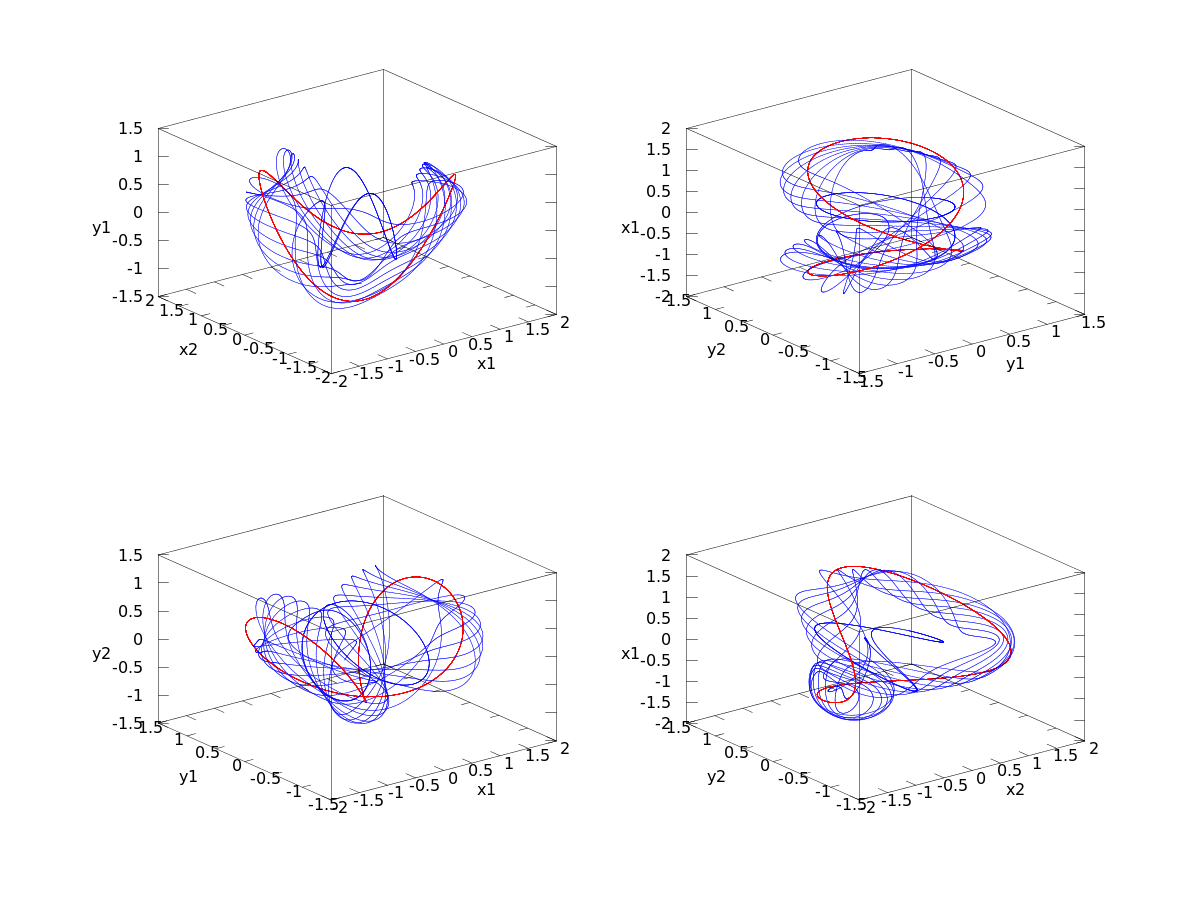
\includegraphics[width=0.9\textwidth]{BBpars3PKflow}
  \end{center}
  \caption{$3D$ projections of trajectories of \twoMode\ flow in full
  \statesp\ for parameters: $\mu_1 = 1.23436,\, a_1=-0.32304,\,
  b_1=-1.07444,\, c_1=1.00000,\, \mu_2=-0.23149,\, a_2=0.44110,\,
  b_2=-0.42287,\, c_2=-1.00000,\, e_2=0.67556$. Blue curve is a
  trajectory starting close to an unstable \reqv, the blue curve in the
  middle of the top left frame, which converges to a stable \rpo, better
  seen in \reffig{fig:BBpars3symmred}. This \rpo\ originates from a Hopf
  bifurcation of a \reqv, here the coexisting attractive \reqv\ plotted
  as red curve.
  }
  \label{fig:BBpars3PKflow}
\end{figure}

\item[2013-08-08  Burak]
According to my simulations, an attracting \eqv\ in the invariant
polynomial basis corresponds to a stable \reqv\ in the full \statesp.
({\bf [2013-08-13 Predrag]} correct.)
Eliminating these parameter values
gives more interesting dynamics.

    \PCedit{
\item[2013-08-13 Predrag] \refFig{fig:BBpars3PKflow} does not look like a
strange attractor. You really want to plot these things in $\{u,v,w,q\}$
representation first, and if something looks chaotic, look at it in a
Poincar\'e section; there it is much easier to see whether there is a
stretch \&\ fold unstable manifold with fractal structure.
    }

\item[2013-08-14 Burak] I am going to try to compute Poincar\'e sections and return maps tomorrow. I have to go back a little bit since my existing Poincare\'e section codes for ChaosBook exercises are extremely sloppy.

\BBedit{
\item[2013-08-19 Burak] Took longer than I thought. I have the \twoMode flow in invariant polynomial basis (\reffig{fig:BBpars4invspacePKflow}), Poincar\'e section and radial return map (\reffig{fig:BBpars4psectnretmap}). Convergence to a periodic orbit is clearly seen on these plots, points with $r=6.8$ mapped on themselves. 
}

\begin{figure}%[ht]
  \begin{center}
  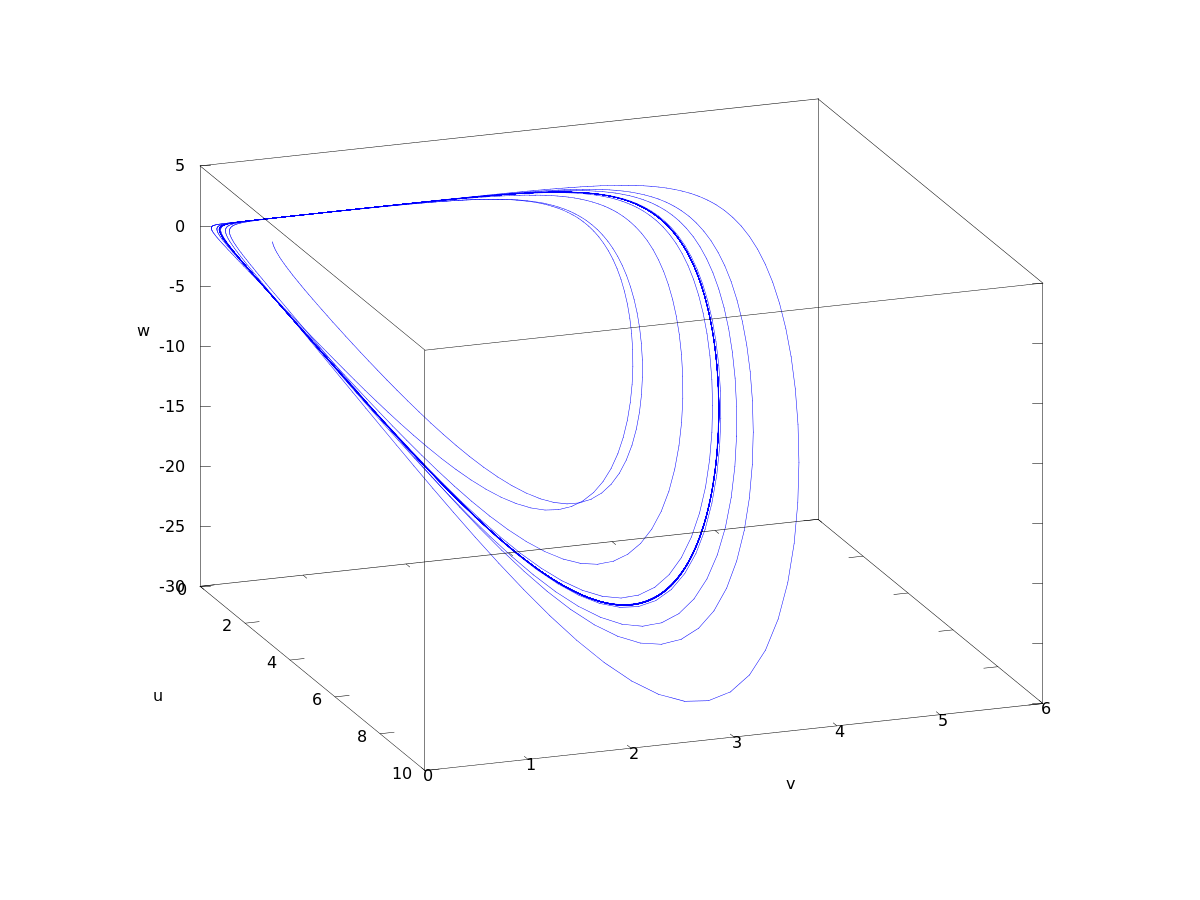
\includegraphics[width=0.6\textwidth]{BBpars4invspacePKflow}
  \end{center}
  \caption{Projections of \twoMode\ dynamics in full \statesp\ and symmetry reduced space. Parameters: $\mu_1 = 1.23436,\,a_1=-0.32304,\,b_1=-1.07444,\,c_1=1.00000,\,\mu_2=-0.23149,\,a_2=0.44110,\,b_2=-0.42287,\,c_2=-1.00000,\,e_2=0.67556$}.
  \label{fig:BBpars4invspacePKflow}
\end{figure}

\begin{figure}%[ht]
  \begin{center}
  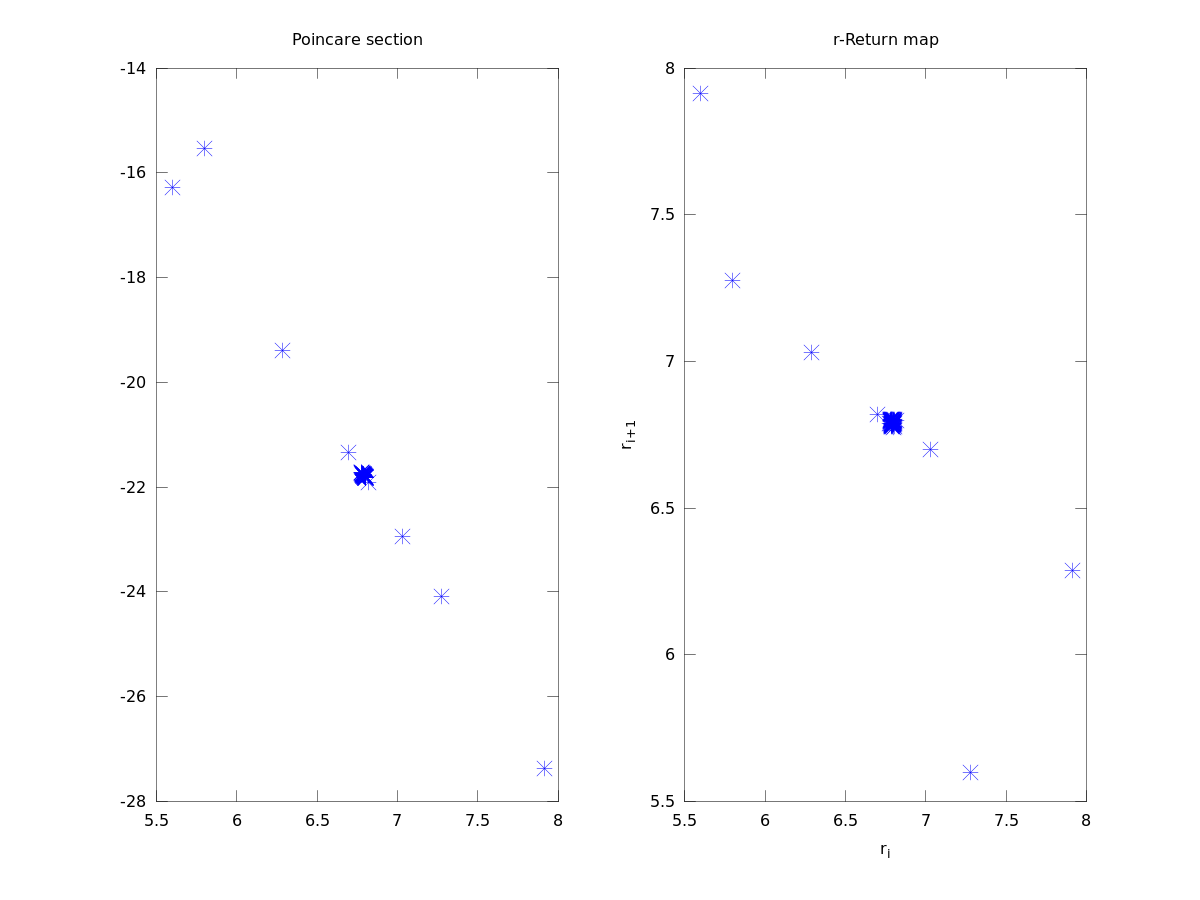
\includegraphics[width=0.9\textwidth]{BBpars4psectnretmap}
  \end{center}
  \caption{Left: Poincar\'e section for the \twoMode\ flow shown in \reffig{fig:BBpars4invspacePKflow}. Poincar\'e hyperplane passes through $\hat{x} = (u=10, v=6, w=0, q=0)$ and the plane normal is $\hat{n} = (-6,10,0,0)$ ($\hat{x}$ rotated 90 degrees about w axis). Right: Poincar\'e return map of radial distance from $w$ axis.}.
  \label{fig:BBpars4psectnretmap}
\end{figure}

\begin{figure}%[ht]
  \begin{center}
  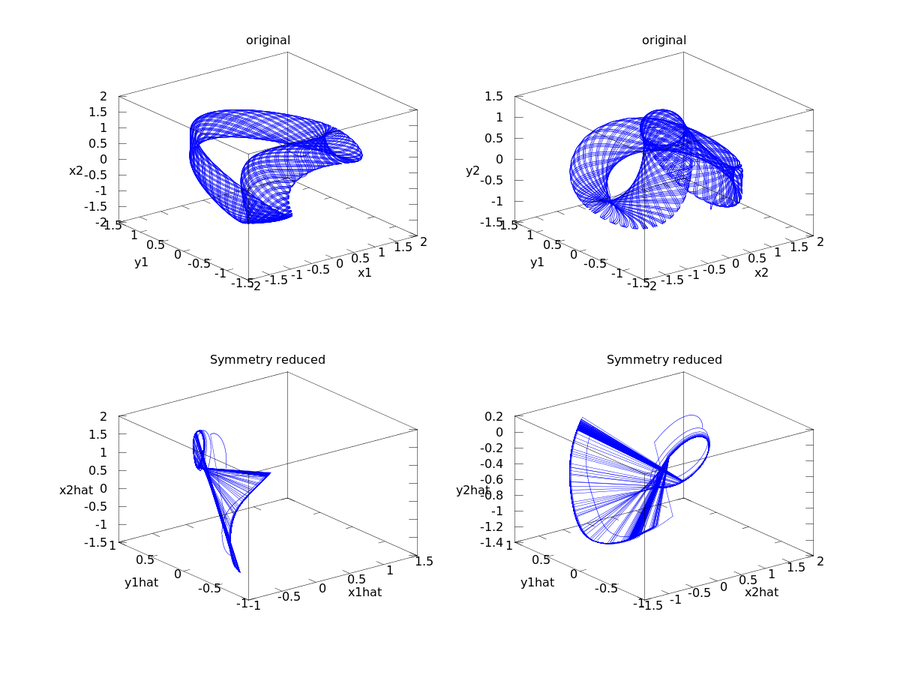
\includegraphics[width=0.9\textwidth]{BBpars3symmred}
  \end{center}
  \caption{Projections of \twoMode\ dynamics in full \statesp\ and symmetry reduced space. Parameters: $\mu_1 = 1.23436,\,a_1=-0.32304,\,b_1=-1.07444,\,c_1=1.00000,\,\mu_2=-0.23149,\,a_2=0.44110,\,b_2=-0.42287,\,c_2=-1.00000,\,e_2=0.67556$}.
  \label{fig:BBpars3symmred}
\end{figure}

\item[2013-08-08  Burak] I think this one (\reffig{fig:BBpars4PKflow}) is chaotic.

\begin{figure}%[ht]
  \begin{center}
  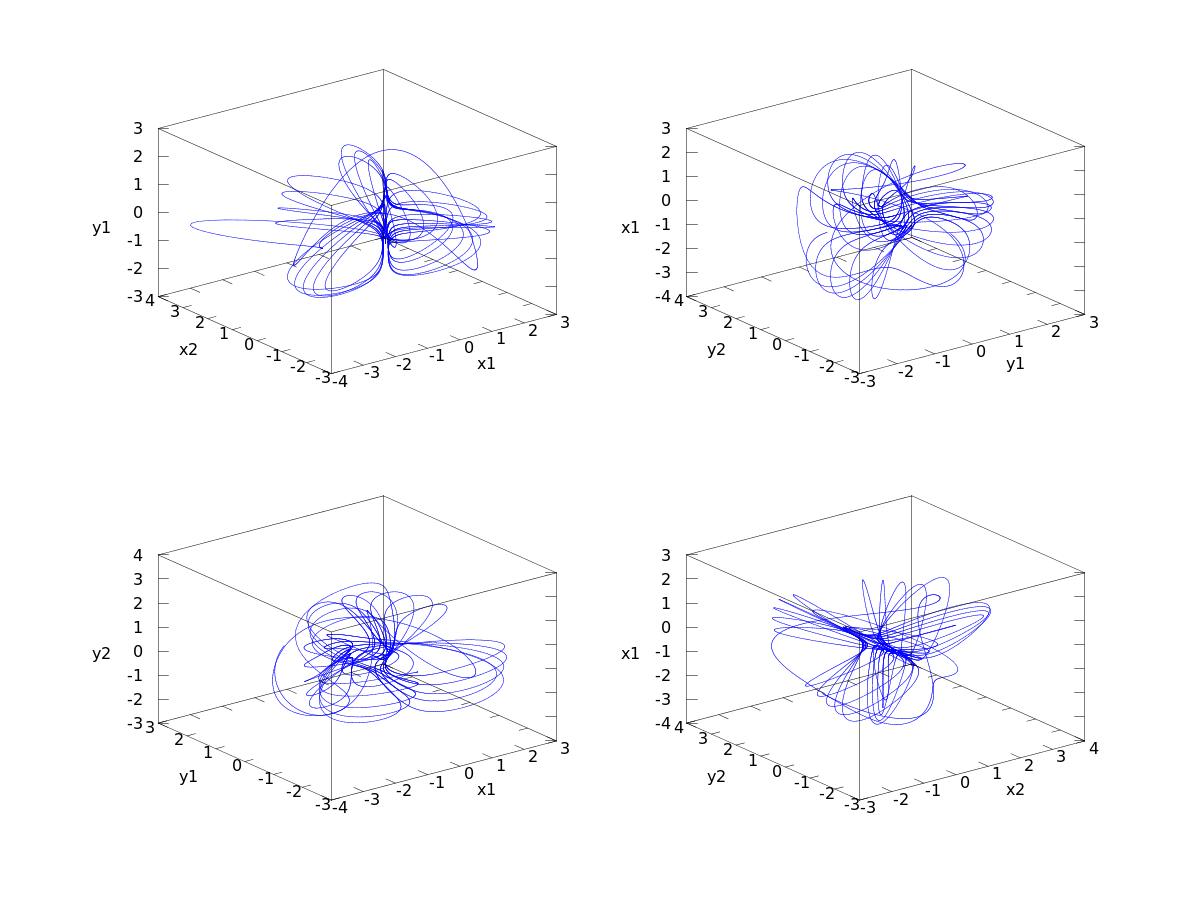
\includegraphics[width=0.9\textwidth]{BBpars4PKflow}
  \end{center}
  \caption{$3D$ projections of trajectories of \twoMode\ flow in full \statesp\ for parameters: $\mu_1 = 1.768907,\,a_1=0.406357,\,b_1=-1.660768,\,c_1=1.00000,\,\mu_2=-0.675565,\,a_2=0.083130,\,b_2=-0.047035,\,c_2=-1.00000,\,e_2=-0.455152$}.
  \label{fig:BBpars4PKflow}
\end{figure}

\item[2013-08-10  Predrag] I think you should cheat and find chaos
    first in the invariant polynomials $\pSRed = \{u,v,w,q\}$ representation -
    that is already symmetry reduced. After it looks chaotic in the
    invariant coordinates, plot the same trajectory in the equivariant
 $\pS = \{x_1,x_2,y_1,y_2\}$ coordinates. That should look messy. After
that construct a \slice\ $\pSRed$.
    \PCedit{
Examples are \reffig{fig:dangelmayrChaos} and \reffig{fig:dangelmayrChaos2}.
    }

That might sound masochistic (why not slice from the start?), but we
are only learning how to slice, and it is easier when you already have a
symmetry-reduced representation. For very high\dmn\ flows we will
not have the luxury of an invariant polynomial basis...

\item[2013-08-12  Burak] I got the parameters that I used in \reffig{fig:BBpars4PKflow} by generating random parameters, discarding if there are attractive equilibria or the time evolution is convergent or divergent in invariant polynomial basis. Unfortunately, this one was a periodic orbit in the invariant polynomial space.

I added another criteria in my parameter generating code on Saturday to eliminate periodic orbits and discovered a bug in it later today. I spent most of today on varying parameters one by one and trying to see if those variations breaks that periodicity. I didn't get anything interesting yet.

I will run another 'new parameter set finder' tonight with the working periodic orbit elimination.

\item[2013-08-13 Predrag] One way to diagnose chaos  is to pick a stable
solution (like \reffig{fig:PKperorb}) and follow it as it undergoes a
Hopf bifurcation into a stable limit cycle. Then one keeps changing
parameters until this \po\ goes unstable and begets chaos, through period
doublings and beyond. To do this, you need to be able to compute Floquet
multipliers of your invariant solutions. For example, does the unstable
\rpo\ in \reffig{fig:BBpars3PKflow} have complex pair of multipliers
(underwent a Hopf bifurcation that turned it unstable) or two real
multipliers (perhaps on the way to period doubling sequence?)

\item[2013-08-13 Predrag] I have asked a Geophysical Fluid Dynamics
(Woods Hole) Fellow Yuuki Yasuda (Earth and Planetary Science, U. Tokyo,
yyuuki@eps.s.u-tokyo.ac.jp) to learn how to use
\HREF{http://sourceforge.net/projects/auto-07p/} {AUTO}, for the same
reason - to follow bifurcations of initially invariant solutions, see how
they go into chaotic behavior. It is well written code which I think is
only good in small dimensions, so we have not used it for our high\dmn\
hydrodynamics calculations. Yuuki will report to me today how it is
working; I'll report whether it might be useful to you.

\item[2013-08-13 Predrag]
I keep getting confused about whether you are plotting a \reqv\ or a \po,
and as we will need this anyhow, please define \eqv, \reqv, \po, and
\rpo\ in \refsect{chap:2modesBBproj}, just to be sure we are on the same
page. (I keep using macros for their names, because depending on the
publication and audience, a `\reqv' might be called a `rotating wave',
etc.)

\item[2013-08-13 Predrag]
A problem with {\twoMode} system is too many parameters (seven! - see
\refeq{PKinvEqs5a}). How about reducing the number of parameters by
demanding that our {\twoMode} system is the $k \in \{\pm 1,\pm 2\}$
truncation of \KS? There is only one parameter left (the system size
$L$), so that is probably too radical -- maybe it will
yield no interesting dynamics at all,
but let something physical like this guide you in reducing the number of
parameters.

The physical setting is that a dissipative turbulent system has a finite
number of Fourier modes nonlinearly coupled and of comparable amplitudes,
while high modes are very strongly suppressed by dissipative terms like
$q_k^4$ in \refeq{BBexpan}. (Xiong Ding can explain the `physical
dimension' to you). So you will be interested in chaotic solutions for
which the two modes $u = {z}_1 \overline{z}_1,\, v = {z}_2
\overline{z}_2$ in \refeq{PKinvEqs1} are of comparable magnitude.

One good exercise is to go through Ruslan's {\em 15.7.1 2009-08-26
Epicycles: 2-Fourier modes} in the \HREF{../blog/blog.pdf} {main blog}.
In this model he looks at a trivial dynamics of two uncoupled modes. I do
not agree with Ruslan pessimistic conclusion - search for `epicycles'
within the blog for more optimistic angles.





\item[2013-08-10  Predrag to Chaos Gang] It's not over until it is over.
\end{description}
